\subsubsection{}
The advantage of alpha-beta pruning algorithm is that it decreases the number of sub-trees explored and leaves evaluated, although the selected move will be the same selected by the minimax algorithm. Therefore, the optimality of the algorithm is maintained, but the runtime is decreased. By pruning branches, and eliminating all the computational cost of their expansion and leaves evaluation, a deeper search can be performed. This advantage is achieved by avoiding searching sub-trees of moves that will not be selected according to the current knowledge of the search tree.

Fig. \ref{fig:3_a_1} shows a scheme of how the alpha-beta pruning algorithm works.
\begin{figure}[h]
    \centering
    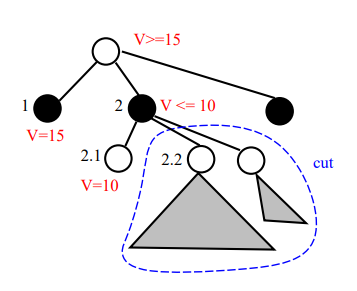
\includegraphics[width=0.5\linewidth]{3_a_1}
    \caption{Explanation of the alpha-beta pruning algorithm (cut-off version).}
    \label{fig:3_a_1}
\end{figure}
The algorithm explanation\footnote{Based on: Hsu TSAN-SHENG, \textit{Alpha-Beta Pruning: Algorithm and Analysis}}, in the cut-off version, follows (it references to Fig. \ref{fig:3_a_1}):
\begin{itemize}
    \item you explore branch at 1 and obtain the best value from it and call it $bound$ (10 in the case of the figure);
    \item You now search the branch at 2 by first searching the branch at 2.1;
    \item branch at 2.1 returns a value that is $\le bound$;
    \item in such a case there is no need to evaluate the branch at 2.2 and all later branches of 2, if any, at all since the best possible value for the branch at 2 must be $\le bound$;
    \item branch 2 cannot return a value better than the one returned from the branch at 1.
\end{itemize}

\subsubsection{}
Optimal pruning happens when the extreme (min or max) value of every node is found first: in nodes where we need to maximize the result, the highest minimax value should be found in the first child; in the nodes where we need to minimize the result, the lowest minimax value should be found in the first child, too.

\subsubsection{}
Fig. \ref{fig:3_0} shows how the algorithm works in practice on the example provided in the handout. No sub-tree or leave is pruned by the algorithm in this case.
\begin{figure}[h]
    \centering
    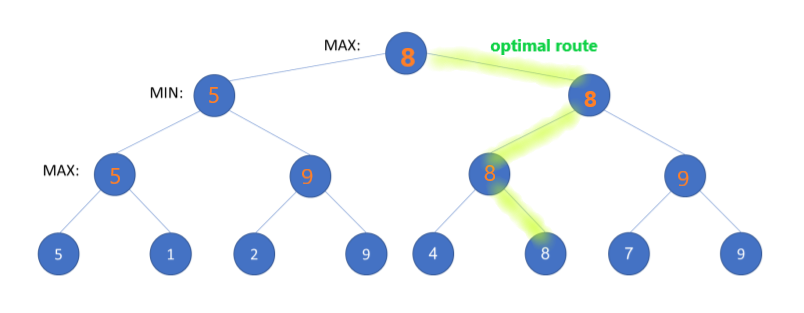
\includegraphics[width=0.6\linewidth]{3_0}
    \caption{Example of pruning according to the alpha-beta pruning algorithm.}
    \label{fig:3_0}
\end{figure}
